%%
%% This is file `sample-xelatex.tex',
%% generated with the docstrip utility.
%%
%% The original source files were:
%%
%% samples.dtx  (with options: `sigconf')
%% 
%% IMPORTANT NOTICE:
%% 
%% For the copyright see the source file.
%% 
%% Any modified versions of this file must be renamed
%% with new filenames distinct from sample-xelatex.tex.
%% 
%% For distribution of the original source see the terms
%% for copying and modification in the file samples.dtx.
%% 
%% This generated file may be distributed as long as the
%% original source files, as listed above, are part of the
%% same distribution. (The sources need not necessarily be
%% in the same archive or directory.)
%%
%% The first command in your LaTeX source must be the \documentclass command.
\documentclass[sigconf]{acmart}

%%
%% \BibTeX command to typeset BibTeX logo in the docs
\AtBeginDocument{%
  \providecommand\BibTeX{{%
    \normalfont B\kern-0.5em{\scshape i\kern-0.25em b}\kern-0.8em\TeX}}}

%% Rights management information.  This information is sent to you
%% when you complete the rights form.  These commands have SAMPLE
%% values in them; it is your responsibility as an author to replace
%% the commands and values with those provided to you when you
%% complete the rights form.
\setcopyright{acmcopyright}
\copyrightyear{2018}
\acmYear{2018}
\acmDOI{10.1145/1122445.1122456}

%% These commands are for a PROCEEDINGS abstract or paper.
\acmConference[Woodstock '18]{Woodstock '18: ACM Symposium on Neural
  Gaze Detection}{June 03--05, 2018}{Woodstock, NY}
\acmBooktitle{Woodstock '18: ACM Symposium on Neural Gaze Detection,
  June 03--05, 2018, Woodstock, NY}
\acmPrice{15.00}
\acmISBN{978-1-4503-XXXX-X/18/06}


%%
%% Submission ID.
%% Use this when submitting an article to a sponsored event. You'll
%% receive a unique submission ID from the organizers
%% of the event, and this ID should be used as the parameter to this command.
%%\acmSubmissionID{123-A56-BU3}

%%
%% The majority of ACM publications use numbered citations and
%% references.  The command \citestyle{authoryear} switches to the
%% "author year" style.
%%
%% If you are preparing content for an event
%% sponsored by ACM SIGGRAPH, you must use the "author year" style of
%% citations and references.
%% Uncommenting
%% the next command will enable that style.
%%\citestyle{acmauthoryear}

%%
%% end of the preamble, start of the body of the document source.
\begin{document}

%%
%% The "title" command has an optional parameter,
%% allowing the author to define a "short title" to be used in page headers.
\title{State of the Art Report - Crowd Simulation}

%%
%% The "author" command and its associated commands are used to define
%% the authors and their affiliations.
%% Of note is the shared affiliation of the first two authors, and the
%% "authornote" and "authornotemark" commands
%% used to denote shared contribution to the research.
\author{Manuel Eiweck}
\affiliation{
	\institution{Student of Technical University Vienna}
}
\email{e1633012@student.tuwien.ac.at}

\author{Bernhard Kerbl}
\affiliation{
	\institution{Institute of Visual Computing \& Human-Centered Technology, Technical University Vienna}
}
\authornote{Advisor}
\email{kerbl@cg.tuwien.ac.at}

%%
%% By default, the full list of authors will be used in the page
%% headers. Often, this list is too long, and will overlap
%% other information printed in the page headers. This command allows
%% the author to define a more concise list
%% of authors' names for this purpose.
\renewcommand{\shortauthors}{Trovato and Tobin, et al.}

%%
%% The abstract is a short summary of the work to be presented in the
%% article.
\begin{abstract}
The goal of this state of the art report is to give a quick overview of the topic. Reader should be able to understand what application areas and research areas are covered, important key concepts and technical terms often used in the field. As crowd simulation is a broad field it is not possible to cover all approaches to a given problem, so there are additional references for further detailed reading. 

In the Introduction key areas, common definitions and terms as well as first research results done in the field are explained. The Report continues with common application areas and an overview of the research areas and the problem these try to solve. After that each area is described in more detail with given approaches. At the end there is a outlook for future research necessary in crowd simulation. 
\end{abstract}

%%
%% The code below is generated by the tool at http://dl.acm.org/ccs.cfm.
%% Please copy and paste the code instead of the example below.
%%
\begin{CCSXML}
<ccs2012>
<concept>
<concept_id>10010147.10010371.10010352</concept_id>
<concept_desc>Computing methodologies~Animation</concept_desc>
<concept_significance>500</concept_significance>
</concept>
<concept>
<concept_id>10010147.10010371.10010352.10010381</concept_id>
<concept_desc>Computing methodologies~Collision detection</concept_desc>
<concept_significance>500</concept_significance>
</concept>
<concept>
<concept_id>10010147.10010371.10010352.10010379</concept_id>
<concept_desc>Computing methodologies~Physical simulation</concept_desc>
<concept_significance>100</concept_significance>
</concept>
<concept>
<concept_id>10010147.10010371.10010352.10010378</concept_id>
<concept_desc>Computing methodologies~Procedural animation</concept_desc>
<concept_significance>500</concept_significance>
</concept>
<concept>
<concept_id>10010147.10010341.10010370</concept_id>
<concept_desc>Computing methodologies~Simulation evaluation</concept_desc>
<concept_significance>300</concept_significance>
</concept>
<concept>
<concept_id>10010147.10010341.10010349.10010359</concept_id>
<concept_desc>Computing methodologies~Real-time simulation</concept_desc>
<concept_significance>500</concept_significance>
</concept>
<concept>
<concept_id>10010147.10010341.10010349.10010362</concept_id>
<concept_desc>Computing methodologies~Massively parallel and high-performance simulations</concept_desc>
<concept_significance>500</concept_significance>
</concept>
</ccs2012>
\end{CCSXML}

\ccsdesc[500]{Computing methodologies~Animation}
\ccsdesc[500]{Computing methodologies~Collision detection}
\ccsdesc[100]{Computing methodologies~Physical simulation}
\ccsdesc[500]{Computing methodologies~Procedural animation}
\ccsdesc[300]{Computing methodologies~Simulation evaluation}
\ccsdesc[500]{Computing methodologies~Real-time simulation}
\ccsdesc[500]{Computing methodologies~Massively parallel and high-performance simulations}

%%
%% Keywords. The author(s) should pick words that accurately describe
%% the work being presented. Separate the keywords with commas.
\keywords{crowd simulation, state of the art report}

%% A "teaser" image appears between the author and affiliation
%% information and the body of the document, and typically spans the
%% page.
\begin{teaserfigure}
  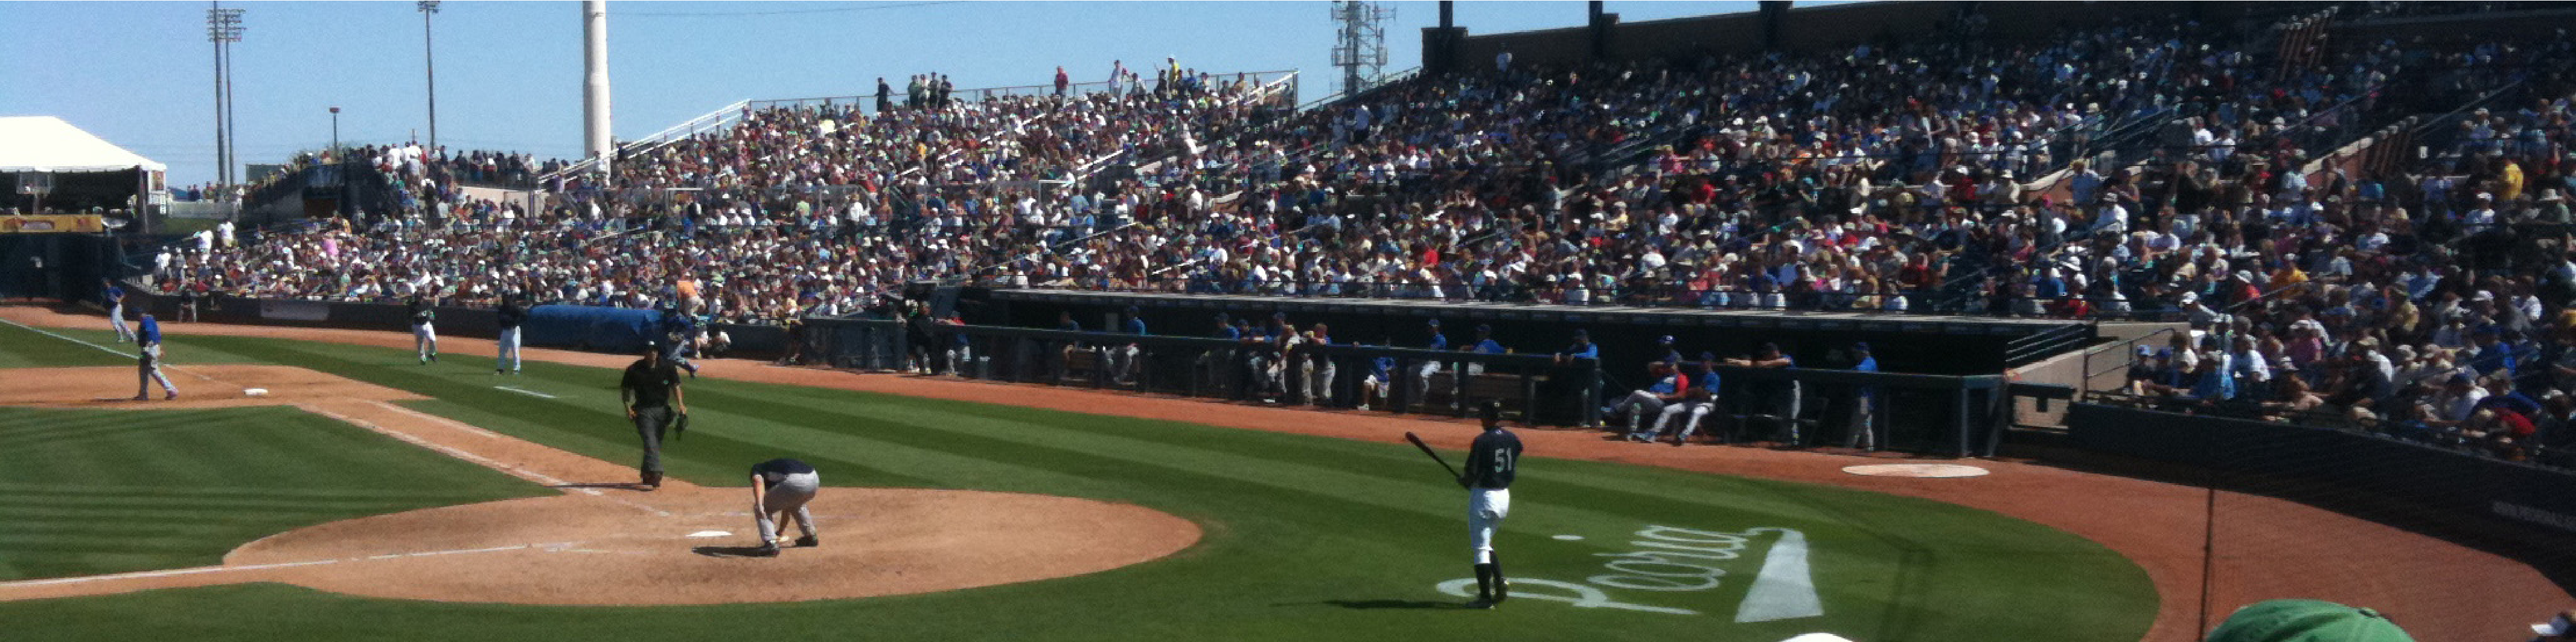
\includegraphics[width=\textwidth]{sampleteaser}
  \caption{Seattle Mariners at Spring Training, 2010.}
  \Description{Enjoying the baseball game from the third-base
  seats. Ichiro Suzuki preparing to bat.}
  \label{fig:teaser}
\end{teaserfigure}

%%
%% This command processes the author and affiliation and title
%% information and builds the first part of the formatted document.
\maketitle

\section{Introduction}

A good comprehensive work on crowd simulation is the book "Crowd Simulation" \cite{thalmann_crowd_2013} in the introduction part I will sum up some key aspects. 

At the beginning some information for the research field in general. The research results in crowd simulation does not come from one or two specific scientific fields or communities, rather the results is a combination of many different fields. A big part comes from the computer graphics field but there is also research done in architecture, physics, robotics, safety science, sociology and so on(TODO: zitat zu werken von den bereichen). A resulting problem is that it is difficult to keep up to date with the current research and because each science field uses different publication methods it is especially easy to overlook some papers on different fields and miss usefully information for the own research. In addition most papers are presenting an solution to a specific problem, for example a pedestrian simulation in real time \cite{karamouzas_predictive_2009},which is not very useful when you want to simulate a big fighting scene in a movie.


\subsection{Key areas}

For a believable crowd simulation there are two parts. First we need to have \textbf{"behavioral animation and environment modeling"}\cite{thalmann_crowd_2013} which defines how the crowd is moving and reacting to each other and the environment. Some example research topic here for example are "Flocks, herds and schools: A distributed behavioral model"\cite{reynolds_flocks_1987} or "Social force model for pedestrian dynamics"\cite{helbing_social_1995}. Second we also need \textbf{"crowd rendering"}\cite{thalmann_crowd_2013} for displaying the large amount of agents in the crowd, where performance is especially important in real time simulations. Crowd rendering also researches the level of detail we are rending, a evacuation simulation could use points or a simple 3D model of a person on the other hand a simulation for movies or games would need more details. Here some examples would be "TODO".

Most application on crowd simulation focus on one of two key areas: 
\begin{itemize}
\item \textbf{"Realism of behavioural Simulation"}\cite{thalmann_crowd_2013} keywords: crowd dynamic, evacuation simulation, social models, collision avoidance and evaluation of results to the real world
\item \textbf{"High quality rendering"}\cite{thalmann_crowd_2013} keywords: crowds in movies and games, performance optimization, combination with motion capturing and physics simulation  
\end{itemize}

\cite{thalmann_crowd_2013}

%%
%% The acknowledgments section is defined using the "acks" environment
%% (and NOT an unnumbered section). This ensures the proper
%% identification of the section in the article metadata, and the
%% consistent spelling of the heading.
\begin{acks}
To Robert, for the bagels and explaining CMYK and color spaces.
\end{acks}

%%
%% The next two lines define the bibliography style to be used, and
%% the bibliography file.
\bibliographystyle{ACM-Reference-Format}
\bibliography{literaturVerzeichnis}

%%
%% If your work has an appendix, this is the place to put it.
\appendix

\end{document}
\endinput
%%
%% End of file `sample-xelatex.tex'.
